\documentclass{beamer}
\usetheme{Berlin}
\usepackage{lipsum}
\usepackage{hyperref}
\usepackage{colortbl}
\usepackage{amsmath,mathtools}
\setbeamercovered{dynamic}

\newtheorem{thm}{Theorem}

\title{My Beamer Assignment}
\subtitle{CS 213, Software Systems Lab}
\author[Karthik Kancharla]{Karthik Kancharla\\
Computer Science and Engineering\\
\texttt{190020020@iitdh.ac.in}}
\institute[CSE, IIT Dharwad]{Indian Institute of Technology, Dharwad}
\logo{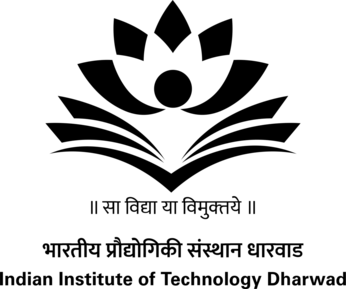
\includegraphics[height = 1cm]{iitdhlogo}}
\date{10th Sept 2020}

\begin{document}
	\frame[plain]{\titlepage}
	\begin{frame}[label = firstframe]
		Hello, this is our first frame. Here you can find info about IIT Dharwad at the below mentioned link.
		\url{www.iitdh.ac.in} or by clicking the following \href{www.iitdh.ac.in}{IIT Dharwad} name.
		\\
		You can find info about super heroes by clicking at the following button.
		\hyperlink{superheroes}{\beamergotobutton{Super Heroes}}\\
		You can find info about mathematicians by clicking the following button.
		\hyperlink{mathematicians}{\beamergotobutton{Mathematicians}}
		
	\end{frame}
	\section{Structures}
	\begin{frame}
		\frametitle{Structures}
		\begin{block}{Theorem: Magic}
			\alt{I have done the magic. You should have trusted me earlier before I have done the magic.}{My name is Alt Temporal. I can do magic by changing myself in different slides.}<2>
		\end{block}
		\begin{alertblock}{The Truth}
			\alt{I was just joking, The above person actually does the magic and also I can do it.}{No don't trust him he doesn't do magic.}<2>
		\end{alertblock}
	\end{frame}
	\begin{frame}
		\frametitle{Structures with columns}
		\begin{columns}
			\begin{column}{0.4\textwidth}
				\begin{alertblock}{Alert Column}
					Remain alert for the red light.
				\end{alertblock}\pause
				\begin{block}{Test your Skills}
					There won't be any blue light at the signal.
				\end{block}
			\end{column}
		\pause
		\begin{column}{0.4\textwidth}
			\begin{exampleblock}{To Go}
				Green light means to go past.
			\end{exampleblock}\pause
			\begin{exampleblock}{Extra Info}
				Green is also the color of this example block.
			\end{exampleblock}
		\end{column}
		\end{columns}
	\end{frame}
	\section{Tables}
		\begin{frame}
		\frametitle{Table Frame 1}
		\begin{table}
			\begin{center}
				\begin{tabular}{ccc}
					\hline
					\multirow{Our Sir in Google Meet}&Student A\pause\\
					&Student B\pause\\
					\hline
					
					Student C&Student D&Student KARTHIK\\
					\hline
				\end{tabular}
			\end{center}
			
			\caption{Google Meet Interface as a Table with Teacher}
		\end{table}
		The table number shows teacher interacting with students in Google Meet interface.\\
	\end{frame}
	\begin{frame}
		\frametitle{Table Frame 2}
		\begin{table}
			
			\begin{center}
				\begin{tabular}{cc}
					\hline
					\multicolumn{2}{c}{Students}\\
					A&B\\
					\hline
					
				\end{tabular}
			\end{center}
			
			\caption{Google Meet Interface without Teacher}
		\end{table}
		The table number shows students in Google Meet interface.
	\end{frame}
	\begin{frame}
		\frametitle{Table Frame 3}
		\begin{table}[h]
			\begin{center}
				\caption{My Sample Table}
				
				\begin{tabular}{l|S|S|r}
					\textbf{Value 1} & \textbf{Value 2} & \textbf{Value 3} & \textbf{Value 4}\\ 
					\hline
					1 & 5 & 6 & 8\pause\\ 
					2 & 9 & 11 & 13\pause\\ 
					3 & 58 & 23 & 62\pause\\ 
				\end{tabular}
			\end{center}
		\end{table}
		This is a sample table consisting of random things
	\end{frame}
\begin{frame}
\frametitle{Table Frame 4}
\begin{table}
\centering
\caption{Students and their Marks}
\begin{tabular}{lc<{\onslide<2->}c<{\onslide<3->}c<{\onslide<4->}c<{\onslide}c}
  Sub & A & B & C & D \\
  Mat     & 35 & 62 & 93 & 24 \\
  Phy     & 32 & 41 & 56 & 96 \\
  Che     &55&83&58&92
\end{tabular}
\end{table}
\end{frame}
	\section{Transitions}
	\begin{frame}
		\frametitle{Transition 1}
		\transdissolve
		\lipsum[1-1]
	\end{frame}
	
	\begin{frame}
		\frametitle{Transition 2}
		\transblindshorizontal
		\lipsum[2-2]
	\end{frame}
	
	\begin{frame}
		\frametitle{Transition 3}
		\transblindsvertical
		\lipsum[3-3]
	\end{frame}
	
	\begin{frame}
		\frametitle{Transition 4}
		\transboxin
		\lipsum[4-4]
	\end{frame}
	\section{Figures}
	\begin{frame}[t]{Great Mathematicians}
		This frame shows pictures of Great Mathematicians.
		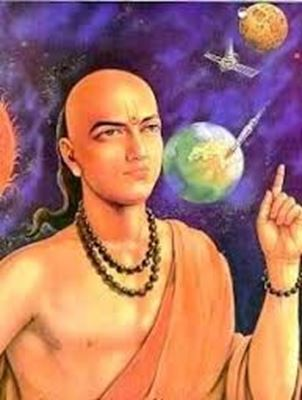
\includegraphics[height = 4cm]{aryabhatta}
		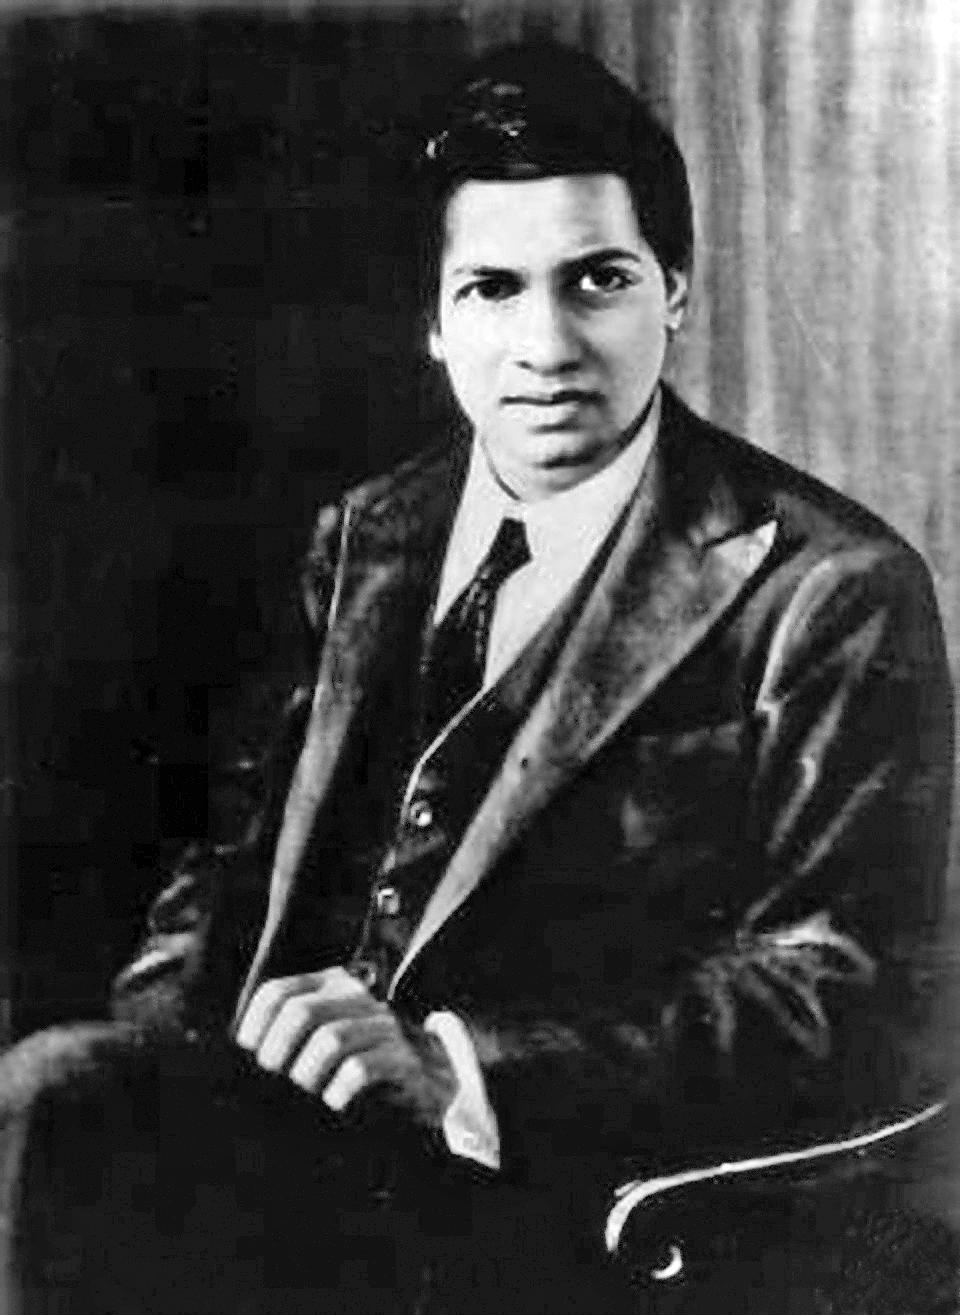
\includegraphics[height = 4cm]{Srinivasa}
	\end{frame}
	\section{Mathematics}
	\begin{frame}
		\frametitle{Mathematics}
		Mathematics is a subject that we learn in the class. This is what you may have known. But it's something else. It's a world of numbers.\\
		\onslide<2->{Mathematics consists of \\}
		\pause 1)Theorem or Proofs\\
		\pause 2)Equations\\
		\onslide<3>{This is the last slide of Mathematics Intro}
	\end{frame}
	\begin{frame}
		\frametitle{Theorems or Proofs 1}
		\begin{block}{Theorem: The Most Complicated One}
			$(a+b)^2=a^2+b^2+2ab$
		\end{block}
		\begin{exampleblock}{Proof:}
			\begin{align}
				(a+b)^2 &= (a+b)(a+b)\nonumber\\
				& = a^2 + ab + ba + b^2\nonumber\\
				& = a^2 + b^2 + 2ab\nonumber
			\end{align}
		\end{exampleblock}
	\end{frame}
\begin{frame}
	\frametitle{Theorems or Proofs 2}
	\begin{block}{Theorem: The Second Most Complicated One}
		$(a-b)^2=a^2+b^2-2ab$
	\end{block}
	\begin{exampleblock}{Proof:}
		\begin{align}
			(a-b)^2 &= (a-b)(a-b)\nonumber\\
			& = a^2 - ab - ba + b^2\nonumber\\
			& = a^2 + b^2 - 2ab\nonumber
		\end{align}
	\end{exampleblock}
\end{frame}
\begin{frame}{Theorem Other Way}
\begin{thm}
Multiplication is not Commutative in Matrices.
\end{thm}
\begin{proof}
    AB is not equal to BA.
\end{proof}
    
\end{frame}
	\begin{frame}
		\frametitle{Equation -1}
		This frame will consist of a multiline equation as follows:\\
		Our Multiline Equation:
		\\
		Area of Circle
		\begin{align}
			A & = {\pi r^2 }\pause\\ \nonumber
			& = \frac{\pi d^2 }{4}
		\end{align}
	\end{frame}
	\begin{frame}
		\frametitle{Equation -2}
		This frame will consist of onemore multiline equation as follows:\\
		Our Multiline Equation:
		\\
		Einstein's Equation
		\begin{align}
			E & = mc^2 \nonumber \\ \nonumber		
		\only<2>{& = (\sqrt{m}c)^2}	
		\end{align}	
	\uncover<1> {See magic converts single line eqn to multi line eqn}
	\\
	\only<2>{See I said no, I know magic, you should agree}
	\end{frame}
	\section{Our Section of Lists}
	\begin{frame}
		\frametitle{Our First List using itemize}
		Hello \pause
		\begin{itemize}
			\item<1-> This is the first list item
			\item<2-> This is the second list item
			\item This is the final list item which will be visible in all slides of the frame
		\end{itemize}
	\end{frame}
	\begin{frame}[label =mathematicians]
		\frametitle{Our Second List using enumerate}
		Well known famous People
		
		\begin{enumerate}[<+->]
			\item \href{https://en.wikipedia.org/wiki/Aryabhata}{Aryabhatta}
			\item \href{https://en.wikipedia.org/wiki/Albert_Einstein}{Einstein}
			\item \href{https://en.wikipedia.org/wiki/Newton}{Newton}
			\item \href{https://en.wikipedia.org/wiki/Niels_Bohr}{Bohr}
			\item \href{www.iitdh.ac.in}{Karthik Kancharla}\\
			You can find more info about them by clicking on their names or by searching at \href{google.com}{Google}
		\end{enumerate}
	\end{frame}
	\begin{frame}[label=superheroes]
		\frametitle{Our Third List using Description}
		\transdissolve
		\begin{description}
		\onslide<2-3>	\item[Iron Man] His speciality is he wears a iron man suit.
		\onslide<3-3>	\item[Thor] He has a hammer.
		\onslide<1-3>	\item[Karthik] He know's how to use Beamer.
		\end{description}
		\alert<3>{Hereby all our lists are also completed}
	\end{frame}
	\begin{frame}
		\frametitle{Our Final Frame that has Different Slides}
		\color<1-2>{blue}{This frame is dedicated to the Beamer and people of IIT Dharwad who are using it.\\}
		\alert<1-2>{This is our final frame, and it says that all the given tasks are completed by:}
		\color<2->{green}{Karthik Kancharla from IIT Dharwad}\\
		To go back to the first frame after title click the following button. \hyperlink{firstframe}{\beamerreturnbutton{Our First Frame}}
	\end{frame}
\end{document}
